\section{Экономический раздел}
\label{sec:economy}

\subsection{Оценка готовности к коммерциализации программной разработки <<Бюро находок>>}

Модель COCOMO II была применена для оценки затрат на разработку и внедрение программного обеспечения. Эта модель является алгоритмической и предназначена для оценки стоимости ПО, обладая рядом преимуществ и содержа проработанные алгоритмы настройки и оценки. COCOMO II использует упрощенную регрессионную формулу, основанную на данных из различных проектов, и поддерживает разнообразные модели жизненного цикла и языки программирования. Оценка трудозатрат и времени, необходимых для разработки, помогает планировать бюджет, определять оптимальные сроки и стоимость внедрения программного продукта.

В модели COCOMO II процесс оценки разделяется на два этапа: предварительная оценка на начальном этапе и более детальная оценка после разработки архитектуры. Для проведения экономического анализа выпускной квалификационной работы применяется предварительная оценка по методике COCOMO II.

Формула~(\ref{eq:pm}) для оценивания трудозатрат (PM) имеет вид:
\begin{equation}\label{eq:pm}
	PM = EAF \times A \times SIZE^E,
\end{equation}
\begin{equation}\label{eq:e}
	E = B + 0.01 \times \sum_{j=1}^{5}SF_j,
\end{equation}
где $B$~--- корректирующий коэффициент. На этапе предварительной оценки его принимают равным 0,91; \\
$А$~--- корректирующий коэффициент. На этапе предварительной оценки его принимают равным 2,94; \\
$SF_j$ (Scale Factors)~--- фактор масштаба; \\
$SIZE$~--– объем программного продукта в тысячах строк исходного текста ($KSLOC$~--- Kilo of Source Line of Code); \\
$EAF$ (Effort Adjustment Factor)~--– произведение выбранных множителей трудоемкости (см. форм. \ref{eq:eaf}):
\begin{equation}\label{eq:eaf}
	EAF = \prod_{i = 1}^{n}EM_i,
\end{equation}
где $EM_i$ (Effort Multiplier)~--- множители трудоемкости. Для предварительной оценки количество факторов в модели равно 8 (n=8). 

\begin{table}[htb]
	\caption{Оценка готовности к коммерциализации}
	\centering
	
	\tolerance=0
	\emergencystretch=10pt
	\hyphenpenalty=0
	\exhyphenpenalty=0
	\begin{tabular}{@{}ll@{}}
		\toprule
		\textbf{Наименование критерия}                       & \textbf{Оценка} \\ \midrule
		Соответствие ожиданиям целевой группы           & 4              \\
		Качество интерфейса                            & 5              \\
		Работоспособность и стабильность               & 4              \\
		Полнота документации                           & 2              \\
		Комплексная безопасность                       & 4              \\
		Ожидаемый эффект от внедрения                  & 4              \\
		Известность бренда производителя               & 1              \\
		Качество сервиса и обслуживания                & 5              \\ \midrule
		Коэффициент степени готовности к коммерциализации & 0,725        \\ \bottomrule
	\end{tabular}
	\label{tab:prepare_mark}
\end{table}

Аргументация оценки готовности к коммерциализации (см. табл. \ref{tab:prepare_mark}):
\begin{itemize}
	\item соответствие ожиданиям целевой группы~--– 4, поскольку в сфере информационной безопасности много направлений, которые невозможно осветить в рамках ознакомительной базы;
	\item качество интерфейса~--– 5, поскольку интерфикс не перегружен и содержит в себе только необходимые элементы управления;
	\item работоспособность и стабильность~--– 4, так как при большой нагрузки на хостинг есть низкая вероятность его отказа;
	\item полнота документации~--– 2, так как документация почти отсутствует (только readme файл и некоторые комментарии к функциям);
	\item комплексная безопасность~--– 4, персональные данные пользователей не хранятся в явном виде на сервере, но абсолютной безопасности не существует; 
	\item ожидаемый эффект от внедрения~--– 4, потому что целевая аудитория была заинтересована проектом во время проведения опроса на ранней стадии разработки;  
	\item известность бренда производителя~--- 1, поскольку это дебютный проект такого масштаба;
	\item качество сервиса и обслуживания~--- 5, поскольку обеспечивается ежедневная проверка электронной почты.
\end{itemize}

Таким образом, коэффициент степени готовности к коммерциализации составляет 0,725 (см форм.~\ref{eq:my_eaf}), что соответствует готовности к выходу на рынок.
\begin{equation}\label{eq:my_eaf}
	EAF = \dfrac{\dfrac{4 + 5 + 4 + 2 + 4 + 4 + 1 + 5}{8} \times 2}{10} = 0{,}725,
\end{equation}

\subsection{Оценка фактора масштаба}

Модель оценки фактора масштаба состоит из следующих факторов:
\begin{itemize}
	\item PREC~--– прецедентность;
	\item FLEX~--– гибкость процесса разработки;
	\item RESL~--– архитектура и разрешение рисков;
	\item TEAM~--– сработанность команды;
	\item PMAT~--– зрелость процессов.
\end{itemize}

\begin{table}[htb]
	\caption{Оценка трудозатрат по разработке ПО согласно модели COCOMO II}
	\centering
	
	\tolerance=0
	\emergencystretch=10pt
	\hyphenpenalty=0
	\exhyphenpenalty=0
	\begin{tabular}{@{}ll@{}}
		\toprule
		\multicolumn{2}{c}{\textbf{Оценка фактора масштаба (j)}} \\
		\midrule
		PREC & 1.24 \\
		FLEX & 2.03 \\
		RESL & 1.41 \\
		TEAM & 1.10 \\
		PMAT & 4.68 \\
		SFj  & 10.46 \\
		E    & 1.0146 \\
		\bottomrule
	\end{tabular}
	\label{tab:labor_costs_cocomo}
\end{table}

Уровни значимости факторов масштаба ($SF_j$) экспертным путем были оценены на следующие значения (см. табл.~\ref{tab:labor_costs_cocomo}):
\begin{itemize}
	\item PREC~--- средний (есть некоторый опыт в продукте и платформе);
	\item FLEX~--- очень высокий (незначительная жесткость процесса);
	\item RESL~--- очень низкий (риски известны на 90%);
	\item TEAM~--- очень высокий (высокая степень взаимодействия);
	\item PMAT~--- высокий.
\end{itemize}

По формуле~\ref{eq:e} имеем:
\begin{equation}\label{eq:eaf}
	E = 0{,}91+0{,}01 \times (1{,}23 + 2{,}03 + 1{,}41 + 1{,}10 + 4{,}68) = 1{,}0146.
\end{equation}

\subsection{Оценка фактора трудоемкости}

Модель оценки фактора трудоёмкости (EMj) состоит из следующих факторов:
\begin{itemize}
	\item PERS~--- квалификация персонала;
	\item PREX~--- опыт персонала;
	\item RCPX~--- сложность и надежность продукта;
	\item RUSE~--- разработка для повторного использования;
	\item PDIF~--- сложность платформы разработки;
	\item FCIL~--- оборудование (инструменты простейшие/интегрированные средства поддержки жизненного цикла);
	\item CSED~--- требуемое выполнение графика работ.
\end{itemize}

Значения множителей приведены в таблице~\ref{tab:labor_costs_factor}.  Основным отличием метода является наличие данных о размере кода (SIZE). Размер продукта может быть определен экспертами с использованием метода PERT или анализа продукта с помощью функциональных точек. Во втором случае размер может быть рассчитан с помощью таблицы \ref{tab:labor_costs_factor}.

\begin{table}[htb]
	\caption{Оценка фактора трудоемкости}
	\centering
	
	\tolerance=0
	\emergencystretch=10pt
	\hyphenpenalty=0
	\exhyphenpenalty=0
	\begin{tabular}{@{}ll@{}}
		\toprule
		\multicolumn{2}{c}{\textbf{Оценка фактора трудоемкости (i)}} \\
		\midrule
		PERS & 0.83 \\
		PREX & 1.00 \\
		RCPX & 1.00 \\
		RUSE & 1.10 \\
		PDIF & 1.00 \\
		FCIL & 1.00 \\
		CSED & 1.00 \\
		EAF  & 0.913 \\
		SIZE & 5.00 \\
		PM   & 13,74 \\
		\bottomrule
	\end{tabular}
	\label{tab:labor_costs_factor}
\end{table}

\begin{equation}\label{eq:my_eaf1}
	EAF = 0{,}83 \times 1 \times 1 \times 1{,}1 \times 1 \times 1 \times 1 = 0{,}913
\end{equation}

\begin{equation}\label{eq:my_pm}
	E = 2{,}94 \times 0{,}913 \times 5 ^ {1{,}0146} = 13{,}74
\end{equation}
Таким образом, полученное значение из расчетов \ref{eq:my_eaf1} и \ref{eq:my_pm} говорит о том, что данный проект может быть выполнен за 13,74 месяца одним человеком.

\subsection{Расчет полной стоимости программного продукта (в части трудозатрат)}

При оценке общей стоимости создания программного продукта важно учитывать не только труд разработчиков, но и различные этапы, включая анализ требований, проектирование функций, архитектуры и интерфейсов, составление документации и плана интеграции, написание кода, тестирование и прочие задачи. В проекте по разработке программного обеспечения задействованы не только программисты, но и тестировщики, дизайнеры, специалисты по внедрению и другие профессионалы. Обычно на каждый час программирования приходится минимум один час работы других специалистов для подготовки и поддержки проекта.

Соотношение зарплат специалистов~[\ref{tab:labor_costs}]:
\begin{itemize}
	\item тестировщики получают 50\% от зарплаты разработчиков;
	\item отдел внедрения получает так же, как и разработчики;
	\item проектировщики – 75\% от вознаграждения разработчиков.
\end{itemize}

\begin{table}[htb]
	\caption{Расчет полной стоимости программного продукта (в части трудозатрат)}
	\centering
	
	\tolerance=0
	\emergencystretch=10pt
	\hyphenpenalty=0
	\exhyphenpenalty=0
	\begin{tabular}{x{3cm}x{3cm}x{3cm}x{3cm}x{3cm}}
		\toprule
		\textbf{Сотрудники (i)} & \textbf{Процент затрат времени на работу i-го специалиста, \%} & \textbf{Трудозатраты, количество мес. PM} & \textbf{Средний оклад, руб.} & \textbf{Приведенные затраты специалистов, руб.} \\ \midrule
		Проектирование (Проектировщик) & 35 & 4,81 & 90000 & 432816,32 \\
		Разработка (Разработчик) & 100 & 13,74 & 120000 & 1648824,08 \\
		Тестирование (Тестировщики) & 50  & 6,87 & 60000 & 412206,02 \\
		Нагрузочное тестирование (Внедрение) & 5 & 0,69 & 120000 & 82441,20 \\
		Внедрение (Внедрение) & 5 & 0,69 & 120000 & 82441,20 \\
		Техническая документация (Производство) & 5 & 0,69 & 60000 & 41220,60 \\
		\multicolumn{4}{l}{\textbf{Итого полная стоимость ПО в части трудозатрат}} & \textbf{2699949,42} \\ 
		\bottomrule
	\end{tabular}
	
	\label{tab:cost_work_time}
\end{table}

Согласно таблице \ref{tab:cost_work_time} получается, что общая сумма затрат на разработку программного продукта, с полным циклом и количеством специалистов равным 6 (i=6), составило 2 млн. 699 тыс. 949 рублей.

\subsection{Оценка стоимости разработки и внедрения программного продукта}

Согласно принятой методике, общая стоимость разработки программного обеспечения включает в себя трудозатраты, к которым добавляется 13\% налога на доходы. Кроме того, следует учесть дополнительные издержки, некоторые из которых являются обязательными, а другие — выборочными.

В деталях:
\begin{itemize}
	\item Возможно начисление бонуса до 15\% от зарплаты за своевременное выполнение задач и удовлетворение требований клиента;
	
	\item Необходимо вычитать 7,6\% из зарплаты на социальное страхование, включая медицинское обеспечение, пенсионные отчисления и социальное страхование;
	
	\item Может быть предусмотрено возмещение расходов на питание в размере 2\% от зарплаты.
\end{itemize}

Кроме того, специалистам необходимо обеспечить рабочее место с современным офисным оборудованием и надежными средствами коммуникации. Работодатель должен заниматься подбором соответствующего персонала, вести финансовый учет через бухгалтерию, обеспечивать порядок в офисе и назначать ответственных за это. Социальный пакет играет ключевую роль, особенно для высококвалифицированных сотрудников.

\begin{table}[htb]
	\caption{Оценка стоимости разработки и внедрения программного продукта}
	\centering
	
	\tolerance=0
	\emergencystretch=10pt
	\hyphenpenalty=0
	\exhyphenpenalty=0
	\begin{tabular}{x{3cm}x{3cm}x{3cm}}
		\toprule
		\textbf{Статьи калькуляции} & \textbf{Процент расходов} & \textbf{Сумма} \\ \midrule
		Полная стоимость ПО в части трудозатрат & {-} & 2699949,425 \\
		Расходы на хозяйственные и административные нужды & 20\%   & 539989,8849 \\
		Премия к заработной плате & 15\%   & 404992,4137 \\
		Компенсация питания сотрудников & 2\%    & 53998,98849 \\
		Взносы на социальное страхование & 7.60\% & 281118,7341 \\
		\multicolumn{2}{l}{\textbf{Полная стоимость внедрения ПО, в т.ч. НДС 0\%}} & \textbf{3980049,446} \\ \bottomrule
	\end{tabular}
	
	\label{tab:calculation_expenses_software_development}
\end{table}

Эти факторы влияют на включение в методику расходов на коммерческую и управленческую деятельность, что составляет около 20\% от общих трудозатрат на разработку программного обеспечения. При определении итоговой стоимости внедрения также следует учесть НДС в размере 20\% от всей суммы. Однако, если программное обеспечение включено в реестр отечественных программ, НДС не взимается. Полная стоимость внедрения данного примера подробно отражена в таблице \ref{tab:calculation_expenses_software_development}.

\subsection{Расчет общего количества капитальных затрат ТСО (CAPEX)}

Согласно методике Gartner по расчету общей стоимости владения (TCO), при определении капитальных затрат учитываются не только затраты на внедрение программного продукта, но и технические, а также консультационные расходы, которые напрямую связаны с установкой и адаптацией системы под нужды компании. Важно также принимать во внимание затраты на обучение сотрудников и приобретение специализированного оборудования и коммуникационных средств для надлежащей работы информационной системы предприятия.

Многие организации не включают эти расходы в проектные затраты, а следовательно, и в общую стоимость продукта, что требует их дополнительного учета при подсчете окончательной суммы капитальных затрат.

Расчет затрат на обучение и переподготовку персонала может быть выполнен следующим образом.

Этот метод считается удобным и доступным для использования, однако его основной недостаток заключается в приблизительности расчетов. Он базируется на анализе множества проектов по разработке и внедрению программного обеспечения в различных, включая иностранные и отечественные, компаниях. Исследования показывают, что затраты на обучение обычно не превышают 20\% от общей стоимости внедрения программного обеспечения.

Таким образом, зная первоначальные капитальные затраты (полная стоимость внедрения программного обеспечения) и максимальный установленный уровень затрат на обучение (20\%), можно определить максимально возможную сумму расходов, которую компания может включить в общую стоимость владения как затраты на обучение и подготовку персонала.

\begin{equation}\label{eq:kpk}
	K_{\text{п.к.}} = 3980049{,}446 \times 20 \% = 796009{,}889
\end{equation}

Таким образом, согласно пропорциональному методу, сумма затрат, выделяемых на обучение персонала, составляет 796 тыс. 9 рублей.

\subsection{Калькуляция затрат на закупку специального оборудования или каналов связи}

\begin{table}[htb]
	\caption{Калькуляция затрат на закупку специального оборудования или каналов связи}
	\centering
	
	\tolerance=0
	\emergencystretch=10pt
	\hyphenpenalty=0
	\exhyphenpenalty=0
	\begin{tabular}{x{5cm}x{3cm}x{3cm}x{3cm}}
		\toprule
		\textbf{Статьи калькуляции} & \textbf{Стоимость оборудования и каналов связи, руб.} & \textbf{Количество, шт} & \textbf{Сумма, руб.} \\ \midrule
		Серверное и сетевое оборудование, СХД & 2000 & 1 & 2000 \\
		Оборудование для информационной безопасности & 0 & 0 & 0 \\
		Платформа виртуализации & 0 & 0 & 0 \\
		Система резервного копирования & 1000 & 1 & 1000 \\
		Интернет с подключением от нескольких провайдеров & 2000 & 1 & 2000 \\
		%Прочее (указать что если есть) & 0 & 0 & 0 \\
		\textbf{ИТОГО на закупку специального оборудования или каналов связи, (Kр), руб} & \multicolumn{3}{c}{\textbf{5000}} \\ 
		\bottomrule
	\end{tabular}
	
	\label{tab:equipment_communication_costs}
\end{table}

При аудите оборудования было выявлено, что для полноценного функционирования ПО необходимо следующее оборудование (см. табл. \ref{tab:equipment_communication_costs}).

\subsection{Расчет общего количества операционных затрат ТСО (OPEX)}

Операционные затраты (форм. \ref{eq:opex})~--- все последующие расходы компании.

\begin{equation}\label{eq:opex}
	OPEX = K_{af} \times T
\end{equation}
где $K_{af}$~--- последующие расходы;; \\
$T$~--- количество лет.

В перечень затрат входят платежи за продление лицензии, обновление программ, внешнее техническое сопровождение, сервисную поддержку, обеспечение безопасности, резервное копирование данных, устранение неполадок, рефакторинг, программирование, поддержание актуальности версий и другие связанные аспекты.

Операционные издержки охватывают расходы на обновление ПО без изменения его функций, управление системами и их поддержку.

Часто компании не принимают во внимание операционные издержки при планировании проектов, что приводит к их отсутствию в общей стоимости продукта. Затраты на обновления, модернизацию и техническую поддержку программного обеспечения оплачиваются заказчиками отдельно, что гарантирует его стабильную работу. Практика показывает, что заказчики чаще всего предпочитают оплачивать техническую поддержку как часть операционных расходов, вместо того чтобы самостоятельно заниматься поддержкой кода.

Для анализа операционных расходов можно провести подробное разделение на разные категории в зависимости от требуемого уровня функциональности и необходимого сопровождения.

Примерный расчет операционных расходов можно выполнить, определив их долю от общей стоимости внедрения программного продукта. Обычно предполагается, что на поддержку и обновление ПО приходится около 30\% от общей суммы расходов в год (см. табл. \ref{tab:cost_summary}).

\begin{table}[htb]
	\caption{Расчет совокупной стоимости владения (СТО)}
	\centering
	
	\tolerance=0
	\emergencystretch=10pt
	\hyphenpenalty=0
	\exhyphenpenalty=0
	\begin{tabular}{x{10cm}x{5cm}}
		\toprule
		\textbf{Статьи затрат} & \textbf{Сумма, руб.} \\ \midrule
		Капитальные затраты  (CAPEX) - первоначальные затраты на приобретение & 4781059,335 \\
		Затраты на внедрение & 3980049,446 \\
		Затраты на обучение персонала & 796009,8892 \\
		Закупка специального оборудования или каналов связи & 5000 \\
		Операционные затраты (OPEX) - эксплуатационные затраты & 3582044,501 \\
		Затраты на обновление и модернизацию (например, продление лицензии, программное обновление) & 398004,9446 \\
		Расходы на управление системой (сопровождение внешнее, сервис поддержки, безопасность, резервное копирование, исправление багов, рефакторинг, исправление кода, поддержка версий) & 796009,8892 \\
		\textbf{Совокупная стоимость владения (ТСО)} & \textbf{8363103,837} \\ \bottomrule
	\end{tabular}
	
	\label{tab:cost_summary}
\end{table}

При запланированном полезном сроке использования ПО в течении 3-x лет, общий объем операционных затрат равен 8363103,837 руб.

\subsection{Расчет совокупной стоимости владения (ТСО)}

Согласно модели расчета ТСО Gartner Group, затраты компании рассчитываются по формуле \ref{eq:tco}:
\begin{equation}\label{eq:tco}
	TCO = CAPEX \times OPEX
\end{equation}

\subsection{Оценка конкурентоспособности программного продукта}

Конкурентоспособность программного продукта определяется его соответствием текущим требованиям рынка и его актуальностью на момент запуска. Для оценки этой конкурентоспособности проводится сравнительный анализ с другими схожими продуктами.

Этот анализ включает оценку того, насколько хорошо продукт соответствует требованиям рынка не только с технической, математической, информационной и организационной точек зрения, но и с коммерческой стороны, включая ценообразование, уровень обслуживания, сеть продаж, рекламу и прочее.

Конкурентоспособность измеряется путем сравнения с аналогичными товарами и рассматривается через призму потребительских интересов, которые можно разделить на объективные и субъективные категории.

К “жестким”, критериям относятся:
\begin{itemize}
	\item Технические характеристики, включая классификацию, производительность и конструктивные особенности продукта;
	\item Эргономические характеристики, связанные с удобством использования и функциональностью;
	\item Качество взаимодействия пользователя с продуктом, скорость утомления, удобство работы и другие аспекты;
	\item Соответствие международным и национальным стандартам, нормативным актам и законодательству.
\end{itemize}

В оценке программного обеспечения по “жестким” критериям ключевыми являются функциональные возможности, как определено в стандарте ГОСТ Р ИСО/МЭК 9126-93, включающем пригодность, корректность, совместимость и защищенность.

“Мягкие” характеристики включают эстетические и визуальные аспекты, такие как дизайн, цвет и упаковка, которые могут влиять на восприятие потребителями. В случае программного обеспечения это может включать настройку интерфейса, интеграцию с удаленными системами и обработку документов.

Также в оценке конкурентоспособности учитываются экономические характеристики, включая начальные и эксплуатационные затраты, которые формируют общую стоимость использования продукта. Эти затраты включают расходы на обновление, апгрейд, управление системой, внешнее обслуживание, техническую поддержку, безопасность, резервное копирование, исправление ошибок и поддержку версий.

Ещё один ключевой элемент, влияющий на конкурентоспособность программного обеспечения, — это организационно-экономические аспекты сделки, включая систему скидок, условия оплаты и доставки, а также гарантийные обязательства. Вначале необходимо определить важность каждого фактора в рамках конкурентоспособности ПО, распределяя веса по аналитическим блокам (согласно таблице \ref{tab:user_characteristics}), при этом суммарный вес факторов в каждом блоке должен составлять 100 процентов.

\begin{table}[htb]
	\caption{Результаты бальной оценки ПО по субъективным пользовательским предпочтениям}
	\centering
	
	\tolerance=0
	\emergencystretch=10pt
	\hyphenpenalty=0
	\exhyphenpenalty=0
	\begin{tabular}{x{5cm}x{2cm}x{2cm}x{2cm}x{2cm}}
		\toprule
		\textbf{Субъективные пользовательские характеристики} & \multicolumn{3}{c}{\textbf{Исследуемые Программные продукты}} & \textbf{Вес критерия} \\ \cmidrule(lr){2-4}
		& \textbf{finds. mirea.ninja} & \textbf{buro-nahodok.ru} & \textbf{buro.nahodok.ru} &                       \\ \midrule
		возможность настройки ПП                              & 5                                & 4                                        & 1                                        & 50                    \\
		возможность работы с территориально-распределенными офисами & 3                          & 5                                        & 1                                        & 25                    \\
		возможность обработки документов                      & 5                                & 3                                        & 3                                        & 25                    \\
		\textbf{Сумма баллов}                                 & \textbf{200}                     & \textbf{200}                             & \textbf{100}                             &                       \\ \midrule
		\textbf{Индекс конкурентоспособности по субъективным пользовательским предпочтениям} & \textbf{1,00} & \textbf{1,00}       & \textbf{0,50}                            &                       \\
		\bottomrule
	\end{tabular}
	\label{tab:user_characteristics}
\end{table}

На следующем этапе требуется собрать данные и провести анализ программного обеспечения и ПО двух основных конкурентов согласно установленным критериям.

В процессе сравнения ПО конкурентов важно оценить соответствие по ряду параметров: сфера применения, объем программных ресурсов, сложность разработки, применение стандартных модулей и типовых решений, затраты труда на разработку, качество результатов, которые предоставляет продукт, время выполнения задач и ценовой уровень. Если прямых аналогов для сравнения нет, следует провести анализ технико-экономических характеристик различных вариантов программного обеспечения или системных компонентов.

Далее осуществляется расчет индексов конкурентоспособности для каждого из определенных блоков.

Используя оценку функциональных возможностей был посчитан индекс конкурентоспособности по функциональным возможностям (см. табл. \ref{tab:functional_capabilities}).

\begin{longtable}{ x{5cm}x{2cm}x{2cm}x{2cm}x{2cm} } 
	
	\caption{Результаты бальной оценки ПО по функциональным возможностям}
	\label{tab:functional_capabilities}
	
	\endfirsthead
	
	\endhead
	
	\endfoot
	
	\endlastfoot
	
	\textbf{Функциональные возможности} & \multicolumn{3}{c}{\textbf{Исследуемые Программные продукты}} & \textbf{Вес критерия} \\ \cmidrule(lr){2-4}
	& \textbf{finds. mirea.ninja} & \textbf{buro-nahodok.ru} & \textbf{buro.nahodok.ru} &                   \\ \midrule
	\multicolumn{5}{@{}l@{}}{\textbf{Пригодность}}                                                                                                               \\
	соответствие назначения целям применения ПС                              & 5                      & 2                       & 4                       & 9                 \\
	соответствие требований к функциям назначению ПС                         & 5                      & 4                       & 4                       & 9                 \\
	соответствие исходной информации требованиям к функциям ПС               & 3                      & 4                       & 2                       & 9                 \\
	соответствие состава и содержания выходной информации для потребителей ПС & 5                    & 3                       & 3                       & 9                 \\
	соответствие структурных характеристик комплекса программ ПС             & 4                    & 3                       & 2                       & 5                 \\
	\midrule\multicolumn{5}{@{}l@{}}{\textbf{Корректность (правильность)}}                                                                                              \\
	соответствие требований к функциям ПС информационной системе              & 5                    & 3                       & 4                       & 2                 \\
	соответствие требований к функциональным компонентам функциям ПС         & 5                    & 5                       & 4                       & 2                 \\
	соответствие текстов программ требованиям к функциональным компонентам   & 5                    & 4                       & 2                       & 2                 \\
	соответствие объектного кода исходному тексту программ                   & 5                    & 4                       & 5                       & 2                 \\
	степень покрытия тестами возможных маршрутов исполнения программ          & 1                    & 2                       & 2                       & 2                 \\
	\midrule\multicolumn{5}{@{}l@{}}{\textbf{Способность к взаимодействию (совместимости)}}                                                                            \\
	с операционной системой                                                  & 1                      & 1                       & 1                       & 5                 \\
	с аппаратной средой                                                      & 1                      & 1                       & 1                       & 5                 \\
	с внешней средой информационной системы и пользователями                 & 5                      & 3                       & 4                       & 5                 \\
	между программными компонентами                                          & 3                      & 1                       & 1                       & 5                 \\
	между компонентами распределенных информационных систем                  & 3                      & 1                       & 1                       & 5                 \\
	\midrule\multicolumn{5}{@{}l@{}}{\textbf{Защищенность}}                                                                                                            \\
	аутентификация элементов систем обработки данных                         & 5                      & 3                       & 5                       & 8                 \\
	управление доступом                                                      & 3                      & 3                       & 3                       & 8                 \\
	протоколирование обращений                                               & 2                      & 3                       & 5                       & 8                 \\
	криптографическая защита                                                 & 4                      & 1                       & 5                       & 0                 \\
	превентивное реагирование                                                & 2                      & 3                       & 3                       & 0                 \\
	\midrule
	\textbf{Сумма баллов}                                                    & \textbf{369}           & \textbf{275}            & \textbf{305}            &                   \\
	\bottomrule
	
\end{longtable}

Аналогично рассчитываются частные индексы по Блокам «Субъективные пользовательские предпочтения» и «Организационные критерии».

Используя оценку функциональных возможностей был посчитан индекс конкурентоспособности по экономическим возможностям (см. табл. \ref{tab:cost_elements}).

\begin{table}[htb]
	\caption{Результаты оценки ПО экономическим критериям (по цене потребления)}
	\centering
	
	\tolerance=0
	\emergencystretch=10pt
	\hyphenpenalty=0
	\exhyphenpenalty=0
	\begin{tabular}{x{5cm}x{2cm}x{2cm}x{2cm}x{2cm}}
		\toprule
		\textbf{Элементы цены потребления} & \multicolumn{3}{c}{\textbf{Исследуемые Программные продукты}} & \textbf{Вес критерия} \\ \cmidrule(lr){2-4}
		& \textbf{finds. mirea.ninja} & \textbf{buro-nahodok.ru} & \textbf{buro.nahodok.ru} &                       \\ \midrule
		\textit{Первоначальные затраты на приобретение}                &                                   &                                         &                                         &                       \\
		Затраты на внедрение                                 & 3.980.049                           & 15.000.000                              & 23.000.000                               & 10                    \\
		Затраты на обучение персонала                        & 796.010                             & 100.000                                 & 100.000                                  & 15                    \\
		Закупка специального оборудования или каналов связи  & 5.000                               & 100.000                                 & 50.000                                   & 10                    \\
		\textit{Эксплуатационные затраты}                             &                                   &                                         &                                         &                       \\
		Затраты на обновление и модернизацию                & 398.005                             & 0                                       & 0                                        & 15                    \\
		Расходы на управление системой                       & 796.010                             & 1.000.000                               & 5.000                                    & 50                    \\
		\textbf{Цена потребления}                            & \textbf{5.975.074}                  & \textbf{16.200.000}                     & \textbf{23.155.000}                      &                       \\ \midrule
		\textbf{Индекс конкурентоспособности по экономическим критериям} & \textbf{1,00} & \textbf{0,37}                           & \textbf{0,26}                            &                       \\
		\bottomrule
	\end{tabular}
	\label{tab:cost_elements}
\end{table}

\subsection*{Вывод}

Основная идея данного подхода заключается в анализе и сравнении основных характеристик товара компании с аналогичными товарами конкурентов, с последующим отображением результатов анализа в виде графика в форме многоугольника. Визуализация конкурентоспособности, созданная на основе данных из таблицы \ref{tab:competitive_indices}, представлена на рисунке \ref{fig:index_diagram}. Можно заметить, что разработанный программный продукт превосходит аналоги и готов к выходу на рынок.

\begin{table}[htb]
	\caption{Расчет итогового рейтинга конкурентоспособности}
	\centering
	
	\tolerance=0
	\emergencystretch=10pt
	\hyphenpenalty=0
	\exhyphenpenalty=0
	\begin{tabular}{x{5cm}x{2cm}x{2cm}x{2cm}x{2cm}}
		\toprule
		\textbf{Частные индексы конкурентоспособности} & \multicolumn{3}{c}{\textbf{Исследуемые Программные продукты}} & \textbf{Вес группы критериев} \\ \cmidrule(lr){2-4}
		& \textbf{finds. mirea.ninja} & \textbf{buro-nahodok.ru} & \textbf{buro.nahodok.ru} &                       \\ \midrule
		Индекс конкурентоспособности по функциональным возможностям                     & 1,00                               & 0,75                                       & 0,83                                       & 40\%                     \\
		Индекс конкурентоспособности по субъективным пользовательским предпочтениям        & 1,00                               & 1,00                                       & 0,50                                       & 15\%                    \\
		Индекс конкурентоспособности по организационным критериям           & 1,00                               & 1,00                                       & 1,00                                       & 15\%                   \\
		Индекс конкурентоспособности по цене потребления      & 1,00                               & 0,37                                       & 0,26                                       & 30\%                     \\
		\textbf{ИТОГОВОЕ ЗНАЧЕНИЕ ИНДЕКСА}              & \textbf{1,00}                    & \textbf{0,71}                            & \textbf{0,63}                             & \textbf{100\%}           \\
		\bottomrule
	\end{tabular}
	\label{tab:competitive_indices}
\end{table}

\begin{figure}[htb]
	\centering
	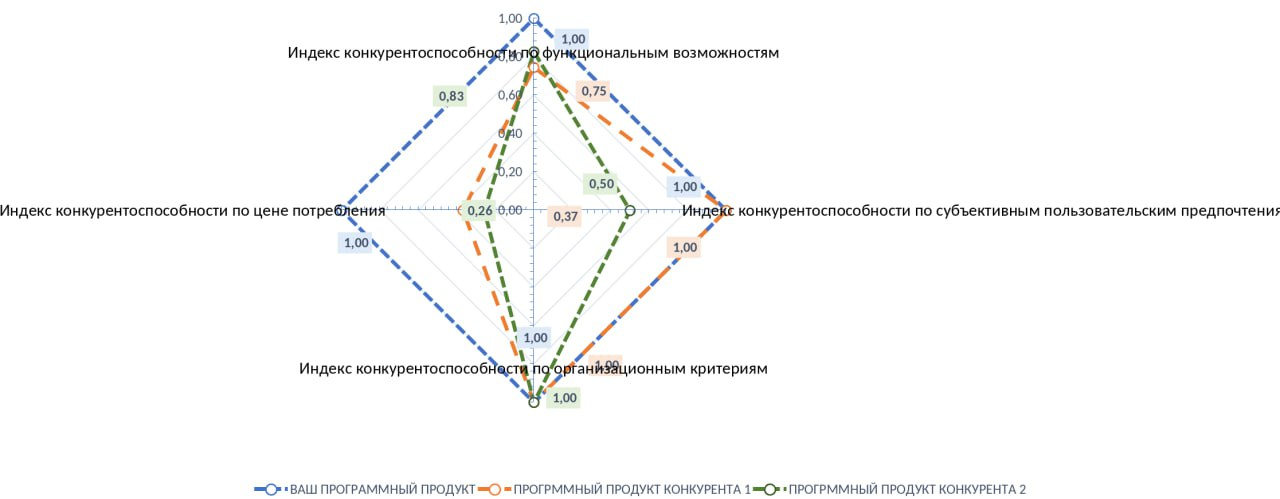
\includegraphics[width=.95\textwidth]{images/kk.jpg}
	\parskip=6pt
	\caption{Рейтинг конкурентоспособности}
	\label{fig:index_diagram}
\end{figure}











\begin{comment}

\subsection{Планирование разработки системы}

Основой данной выпускной квалификационной работы является <<Разработка системы для поиска и возврата утерянных вещей>>. В данном разделе определяются уровень сложности и затраты на создание программного и аппаратного обеспечения, а также оценивается экономическая выгода, которую можно получить от использования разрабатываемого программного обеспечения.

\subsubsection{Определение трудоемкости и продолжительности работ по созданию УСПД}

В этом разделе определяются уровень сложности и затраты на создание программного и аппаратного обеспечения, а также проводится оценка экономической выгоды от использования разрабатываемого ПО. Процесс разработки включает анализ предметной области, имитационный анализ, создание, настройку и тестирование системы.

\begin{itemize}	
	\item Техническое задание. Регламентированы следующие этапы исследования: составление технического задания, включающего формулировку задач, подбор литературы, сбор исходных данных, определение системных требований, а также определение этапов, фаз и сроков разработки программного обеспечения.
	
	\item Эскизный проект. Этот этап включает в себя использование программных средств для анализа схожих тем, разработки общих программных структур и структур по подсистемам, создания прототипов и документации.
	
	\item Технический проект. Этот этап включает в себя определение требований к программному обеспечению и выбор инструментов и использование программных средств.
	
	\item Рабочий проект. Этап включает компоновку и дизайн, программирование, тестирование и отладку ПО, проектирование плат, а также координацию и утверждение работоспособности всей системы.
	
	\item Внедрение. Подразумевает под собой использование на реальной инфраструктуре; анализ полученных данных в результате исследований, благодаря которым можно будет скорректировать техническую документацию.
\end{itemize}

Трудоемкость работ по созданию программного обеспечения носит вероятностный характер, поскольку определяется суммой сложности этапов и видов работ, оцениваемых экспертами в ручные дни, и зависит от многих факторов, которые трудно учесть.

Трудоемкость каждого вида работ определяется по формуле~(\ref{eq:t_i}).
\begin{equation}\label{eq:t_i}
	t_i=\frac{3 \cdot t_{min} + 2 \cdot t_{max}}{5},
\end{equation}
где $t_{min}$~--- минимально возможная трудоемкость выполнения отдельного вида работ; \\
$t_{max}$~--- максимально возможная трудоемкость выполнения отдельного вида
работ.

Различные виды работ имеют свою продолжительность в календарных днях ($T_{i}$), определяясь по формуле~(\ref{eq:T_i}), в днях:
\begin{equation}\label{eq:T_i}
	T_i=\frac{t_{i}}{\text{Ч}_{i}} \cdot K_{\text{вых}},
\end{equation}
где $t_{i}$~--- трудоемкость работ, человеко-дней; \\
$\text{Ч}_{i}$~--- численность исполнителей, человек; \\
$K_{\text{вых}}$~--- коэффициент, учитывающий выходные и праздничные дни, находится по формуле~(\ref{eq:k_vih}):
\begin{equation}\label{eq:k_vih}
	K_{\text{вых}}=\frac{K_{\text{кал}}}{K_{\text{раб}}},
\end{equation}
где $K_{\text{кал}}$~--- календарные дни; \\
$K_{\text{раб}}$~--- рабочие дни; \\
$K_{\text{вых}}$~--- 1,48.

Далее предоставляется перечень разновидностей и стадий рабочей деятельности по разработке ПО, экспертные оценки, а также рассчитываемые переменные их трудоемкости, а также продолжительность каждого вида работ, рассчитанные по формулам~(\ref{eq:t_i}) и~(\ref{eq:T_i}), представлены в таблице~\ref{tab:work_hours}.

\begin{longtable}{ |x{1cm}|x{3cm}|x{1cm}|x{1cm}|x{1cm}|x{3cm}|x{3cm}| } 
	
	\caption{Расчет трудоемкости и продолжительности работ по созданию ПО и аппаратных средств календарных дней}
	\label{tab:work_hours} \\ 
	
	\hline 
	\parbox[t]{2mm}{\multirow{2}{*}{\rotatebox[origin=c]{90}{\bfseries \textnumero{} работы\hspace{5mm}}}} &
	\multicolumn{1}{p{3cm}|}{\multirow{2}{*}{\parbox{3cm}{\bfseries Стадии разработки}}} & 
	\multicolumn{3}{p{3cm}|}{\bfseries Трудоемкость, чел. дни} & 
	\multicolumn{1}{p{3cm}|}{\bfseries Количество работников, чел.} & 
	\multicolumn{1}{p{3cm}|}{\bfseries Про\-дол\-жи\-тель- ность работ, календарные дни}
	
	\endfirsthead
	
	
	\multicolumn{7}{l}{{Продолжение таблицы \thetable{}.}} \\ \hline
	\parbox[t]{2mm}{\multirow{2}{*}{\rotatebox[origin=c]{90}{\bfseries \textnumero{} работы\hspace{5mm}}}} &
	\multicolumn{1}{p{3cm}|}{\multirow{2}{*}{\parbox{3cm}{\bfseries Стадии разработки}}} & 
	\multicolumn{3}{p{3cm}|}{\bfseries Трудоемкость, чел. дни} & 
	\multicolumn{1}{p{3cm}|}{\bfseries Количество работников, чел.} & 
	\multicolumn{1}{p{3cm}|}{\bfseries Про\-дол\-жи\-тель- ность работ, календарные дни}
	\endhead
	
	\endfoot
	
	\endlastfoot
	
	\hline
	
	&& $t_{min}$ & $t_{max}$ & $t_{i}$ & $\text{Ч}_i$ & $T_i$ \\ \hline
	
	\multicolumn{7}{|c|}{Техническое задание} \\ \hline
	
	1 & - постановка задачи & 3 & 6 & 4.2 & 1 & 6.2 \\ \hline
	
	2 & - подбор литературы & 2 & 3 & 2.4 & 1 & 3.6 \\ \hline
	
	3 & - сбор исходных данных & 4 & 5 & 4.4 & 1 & 6.5 \\ \hline
	
	4 & - определение требований к системе & 3 & 4 & 3.4 & 1 & 5.0 \\ \hline
	
	5 & - определение стадий, этапов и сроков разработки ПО & 2 & 3 & 2.4 & 1 & 3.6 \\ \hline
	
	\multicolumn{7}{|c|}{Эскизный проект} \\ \hline
	
	6 & - анализ программных средств схожей тематики & 7 & 8 & 7.4 & 1 & 11.0 \\ \hline
	
	7 & - разработка общей структуры ПО & 4 & 8 & 5.6 & 1 & 8.3 \\ \hline
	
	8 & - разработка структуры программы и подсистем & 5 & 8 & 6.2 & 1 & 9.2 \\ \hline
	
	9 & - создание прототипа & 4 & 6 & 4.8 & 1 & 7.1 \\ \hline
	
	10 & - документирование & 2 & 3 & 2.4 & 1 & 3.6 \\ \hline
	
	11 & - определение требований к ПО & 3 & 4 & 3.4 & 1 & 5.0 \\ \hline
	
	12 & - выбор инструментальных средств & 3 & 4 & 3.4 & 1 & 5.0 \\ \hline
	
	\multicolumn{7}{|c|}{Рабочий проект} \\ \hline
	
	13 & - программирование & 20 & 25 & 22 & 1 & 32.6 \\ \hline
	
	14 & - тестирование и отладка ПО & 7 & 8 & 7.4 & 1 & 11.0 \\ \hline
	
	15 & - разработка программной документации & 4 & 6 & 4.8 & 1 & 7.1 \\ \hline
	
	16 & - согласование и утверждение работоспособности системы & 2 & 3 & 2.4 & 1 & 3.6 \\ \hline
	
	\multicolumn{7}{|c|}{Внедрение} \\ \hline
	
	17 & - опытная эксплуатация & 6 & 8 & 6.8 & 1 & 10.1 \\ \hline
	
	18 & - анализ данных, полученных в результате эксплуатации & 2 & 4 & 2.8 & 1 & 4.1 \\ \hline
	
	19 & - корректировка технической документации по результатам испытаний & 1 & 2 & 1.4 & 1 & 2.1 \\ \hline
	
	& {\bfseries Общая трудоемкость разработки} &&& 98 && 144 \\ \hline
\end{longtable}

Следовательно, общая продолжительность проведения работ $T_{i} = 144$.

\subsubsection{Построение ленточного графика проведения исследования}

В качестве инструмента планирования используется ленточный график~(\ref{fig:work_waterfall}).
\begin{figure}[H]
	\centering
	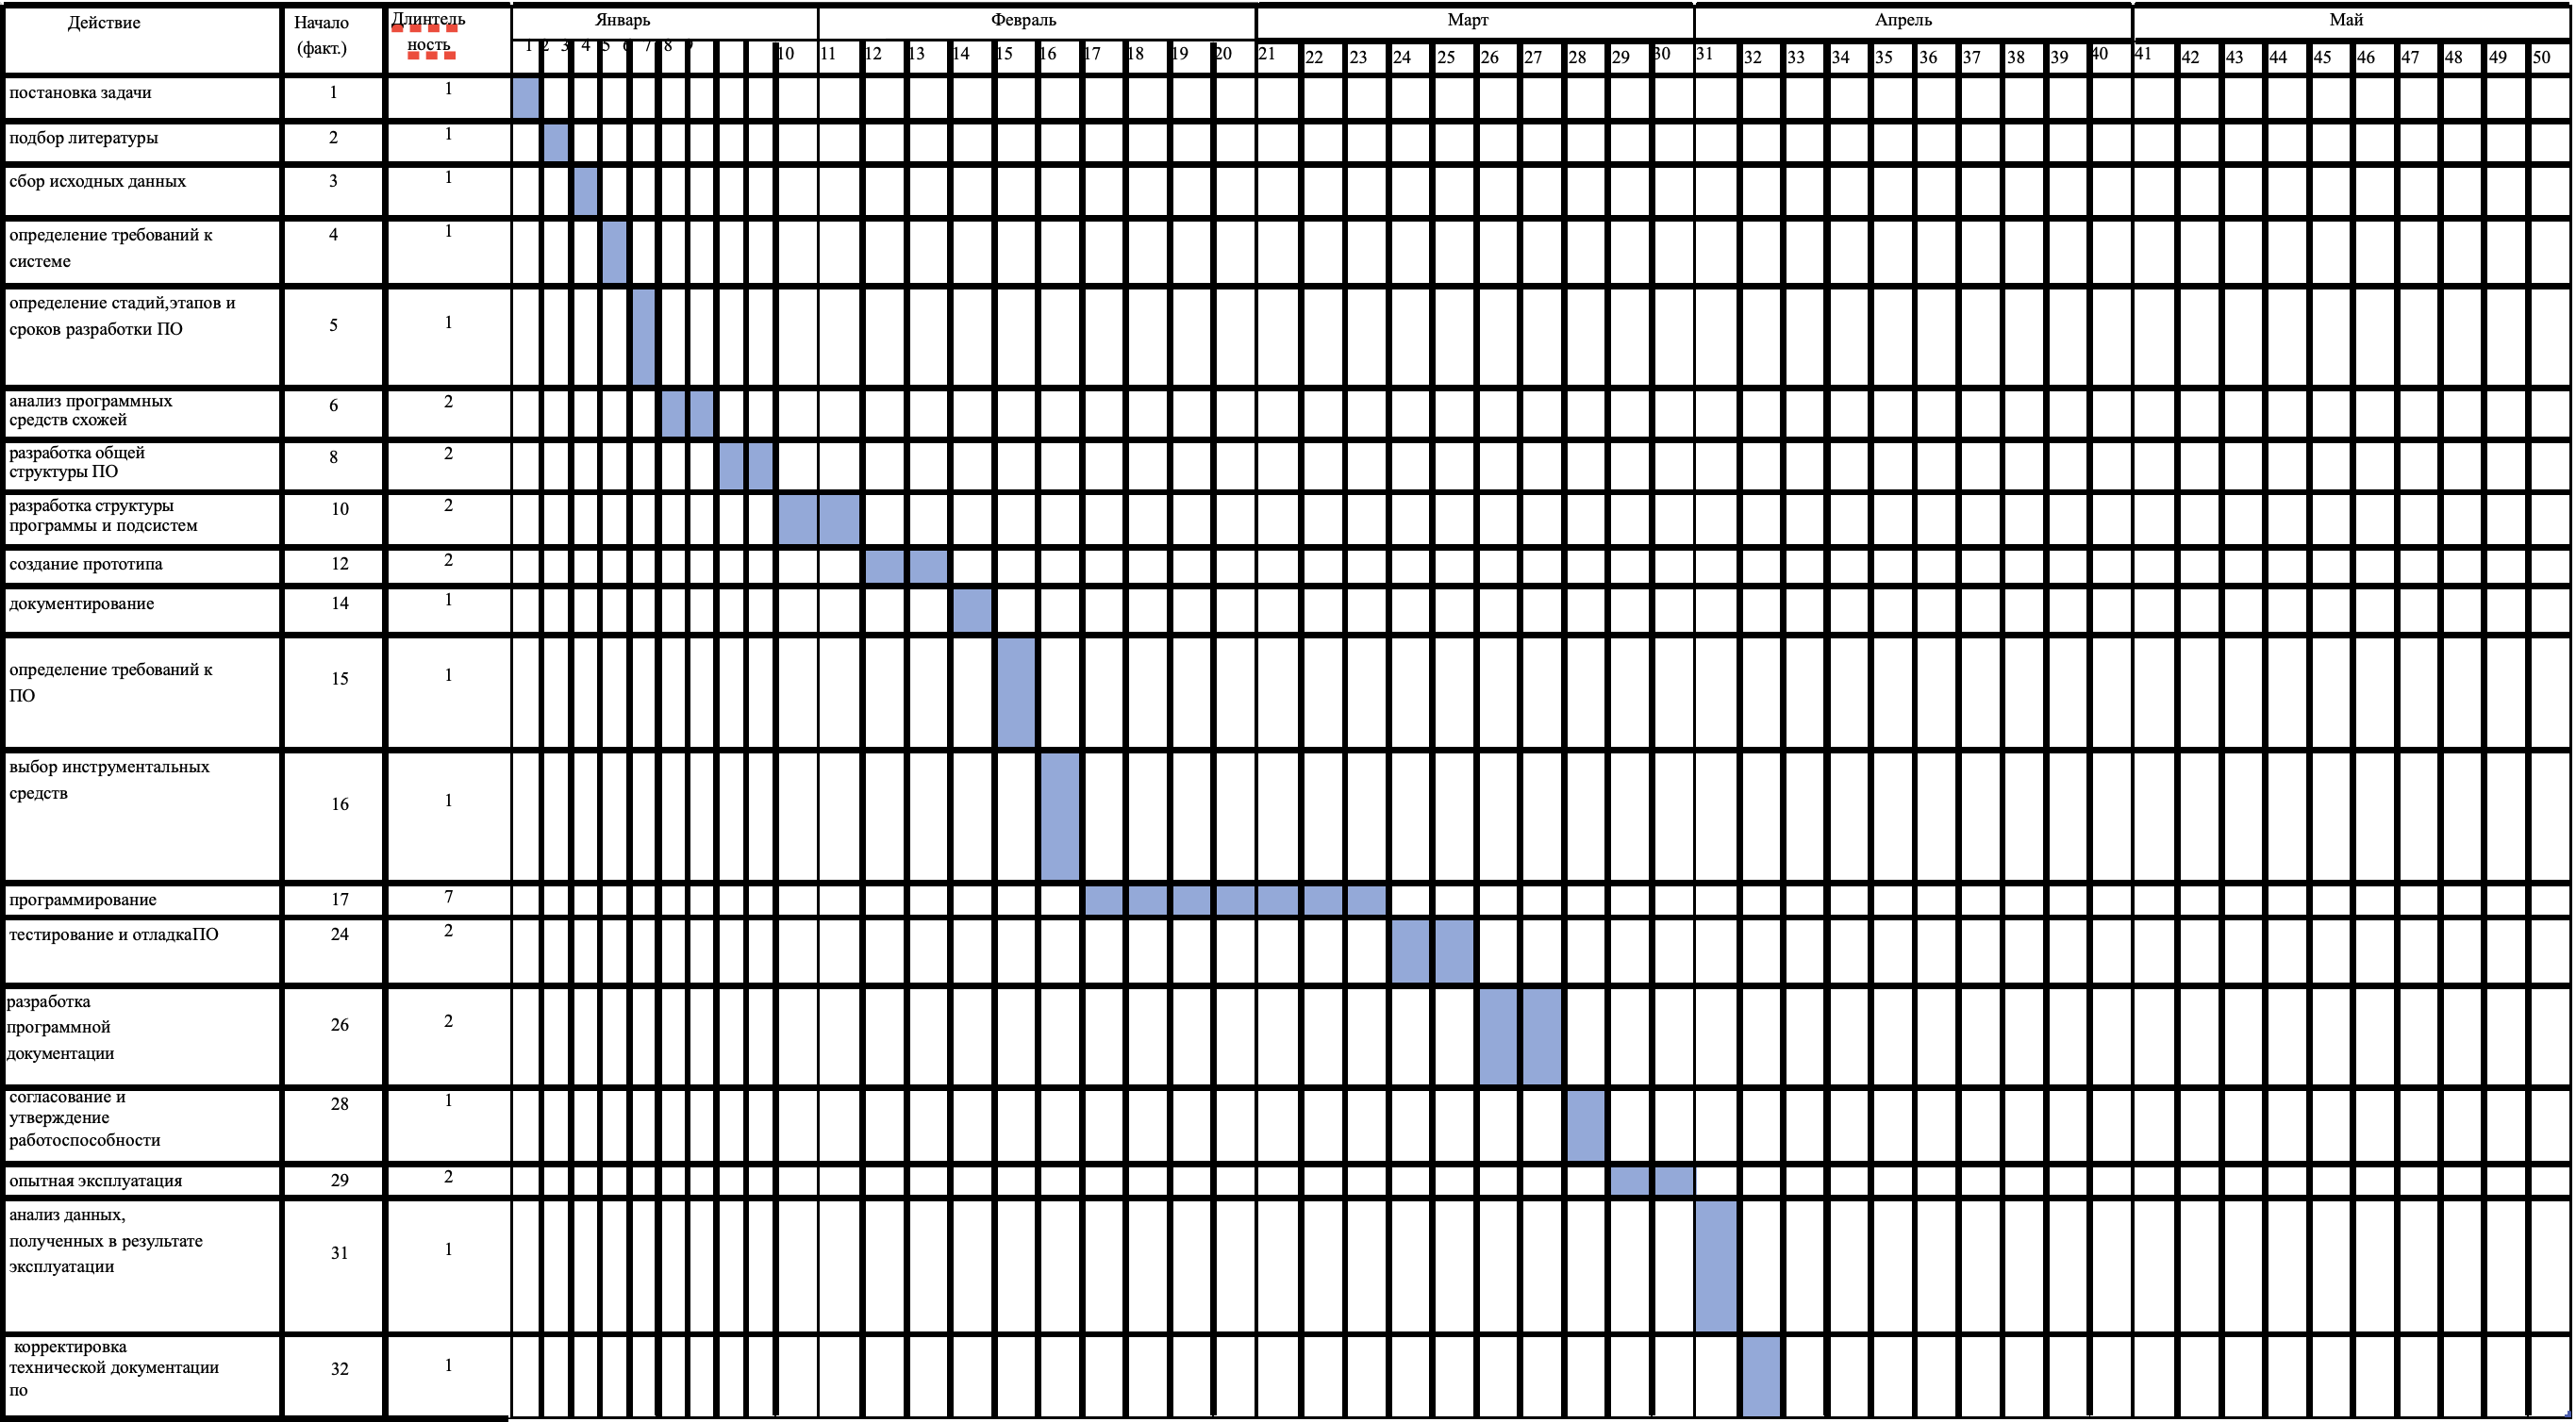
\includegraphics[width=.7\textheight,angle=90,origin=c]{images/work_waterfall}
	\parskip=6pt
	\caption{Ленточный график}
	\label{fig:work_waterfall}
\end{figure}

Подобный график позволяет наглядно представить логическую
последовательность и взаимосвязь отдельных работ. График представляет собой
таблицу с перечислением названий стадий разработки, видов работ, длительность выполнения работ. Данный график построен по данным таблицы~\ref{tab:work_hours}. В этом графике временная единица выполнения работ оценивается в 3 дня.

\subsection{Расчет сметы затрат на разработку представленной работы}

Сметная стоимость проектирования и внедрения программы включает в себя затраты, определяемые по формуле~(\ref{eq:estimate}):
\begin{equation}\label{eq:estimate}
	C_{\text{пр}} = C_{\text{осн}} + C_{\text{доп}} + C_{\text{соц}} + C_{\text{м}} + C_{\text{маш.вр}} + C_{\text{н}},
\end{equation}
где $C_{\text{пр}}$~--- стоимость разработки ПО; \\
$C_{\text{осн}}$~--- основная заработная плата исполнителей; \\
$C_{\text{доп}}$~--- дополнительная заработная плата исполнителей, учитывающая потери времени на отпуска и болезни (принимается в среднем 10\% от основной заработной платы; \\
$C_{\text{соц}}$~--- отчисления в фонд социального страхования – 30\% от основной и дополнительной заработной платы; \\
$C_{\text{м}}$~--- затраты на используемые материалы; \\
$C_{\text{маш.вр}}$~--- стоимость машинного времени; \\
$C_{\text{н}}$~--- накладные расходы включают затраты на управление, уборку, ремонт, электроэнергию, отопление и др. (принимаются в размере 60\% от основной и дополнительной заработной платы).

\subsubsection{Основная заработная плата исполнителей}

На статью «Заработная плата» относят заработную плату научных, инженерно-технических и других работников, непосредственно участвующих в разработке ПО. Расчет ведется по формуле (\ref{eq:salary}):

\begin{equation}\label{eq:salary}
	\text{З}_{\text{исп}} = \text{З}_{\text{ср}} \cdot T,
\end{equation}
где $\text{З}_{\text{исп}}$~--- заработная плата исполнителей (руб.); \\
$\text{З}_{\text{ср}}$~--- средняя тарифная ставка работника организации разработчика ПО (руб./чел./дни); \\
$T$~--- трудоемкость разработки ПО (чел.дни).

$\text{З}_{\text{ср}}$ определяется по формуле~(\ref{eq:work_tariff}):
\begin{equation}\label{eq:work_tariff}
	\text{З}_{\text{ср}} = \frac{C}{\text{Ф}_{\text{мес}}},
\end{equation}
где $C$~--- зарплата труда на текущий момент времени (руб./мес.); \\
$\text{Ф}_{\text{мес}}$~--- месячный фонд рабочего времени исполнителя (дни).

Затраты на статью <<Заработной платы>> приведены в таблице~\ref{tab:salary}.
\begin{table}[htb]
	\caption{Затраты на заработную плату}
	\centering
	
	\tolerance=0
	\emergencystretch=10pt
	\hyphenpenalty=0
	\exhyphenpenalty=0
	\begin{tabular}{ |x{1cm}|x{2cm}|x{2cm}|x{2cm}|x{3cm}|x{2cm}| } 
		\hline
		\textnumero{} & Исполнитель & Оклад, руб./мес. & Оклад, руб./мес. & Трудоемкость, чел.дни & Сумма, руб. \\ \hline
		
		1 & Инженер-программист & 70000 & 3500 & 98 & 343000 \\ \hline
		
		\multicolumn{4}{|x{7cm}|}{Общая основная заработная плата исполнителей, $C_{\text{осн}}$} & 98 & 343000 \\ \hline
		
	\end{tabular}
	\label{tab:salary}
\end{table}

\subsubsection{Дополнительная заработная плата исполнителей}

Дополнительная заработная плата на период разработки ПО рассчитывается относительно основной и составляет 10\% от её величины, рассчитывается по формуле~\ref{eq:addit_salary}.
\begin{equation}\label{eq:addit_salary}
	C_{\text{доп}} = C_{\text{осн}} \cdot 0{,}1 = 34300\,\text{(руб. )}.
\end{equation}

\subsubsection{Расчет отчислений на социальное страхование}

Отчисления на социальное страхование рассчитываются относительно выплаченной заработной платы по формуле~(\ref{eq:social_pay}). Составляют 30%:
\begin{equation}\label{eq:social_pay}
	\begin{array}{l}
		C_{\text{соц}} = ( C_{\text{доп}} + C_{\text{доп}} ) \cdot 0{,}3 \\ 
		C_{\text{соц}} = (34300 + 343000) \cdot 0{,}3 = 113190\,\text{(руб. )}
	\end{array}
\end{equation}

На эту статью относят все затраты на магнитные носители данных, бумагу, для печатных устройств, канцтовары и др. Затраты по ним определяются по экспертным оценкам. Расчет расходов на материалы приведен в таблице~\ref{tab:additional_pay}.

\begin{table}[htb]
	\caption{Расчёт расходов на материалы}
	\centering
	
	\tolerance=0
	\emergencystretch=10pt
	\hyphenpenalty=0
	\exhyphenpenalty=0
	\begin{tabular}{ |x{1cm}|x{4cm}|x{4cm}|x{4cm}| } 
		\hline
		\textnumero{} & Материалы & Количество, штуки & Стоимость, рубли \\ \hline
		
		1 & Бумага писчая, листов & 1000 & 800 \\ \hline
		
		2 & Картридж для принтера, шт. & 1 & 1000 \\ \hline
		
		3 & Другие канцтовары & - & 1000 \\ \hline
		
		\multicolumn{3}{|x{12cm}|}{Общая стоимость материалов, $C_{м}$} & 2800 \\ \hline
		
	\end{tabular}
	\label{tab:additional_pay}
\end{table}

\subsubsection{Накладные расходы}

На статью «Накладные расходы» относят расходы, связанные с управлением и организацией работ. Накладные расходы рассчитываются относительно основной заработной платы. Величина накладных расходов принимается равной 60~\% от основной зарплаты исполнителей. Формула расчета~(\ref{eq:overheads}):
\begin{equation}\label{eq:overheads}
	C_{\text{н}} = C_{\text{осн}} \cdot K,
\end{equation}
где $C_{\text{н}}$~--- накладные расходы; \\
$C_{\text{осн}}$~--- основная заработная плата исполнителей; \\
$K$~--- коэффициент учета накладных расходов.

\begin{equation*}
	C_{\text{н}} = 343000 \cdot 0{,}6 = 205800\,\text{(руб.)}
\end{equation*}

\subsubsection{Расчет стоимости машинного времени}

Затраты на машинное время, необходимое для разработки ПО, расходы на приобретение и подготовку материалов научно-технической информации, расходы на использование средствами связи. Расчет затрат на машинное время осуществляется по формуле~(\ref{eq:machine_pay}):

\begin{equation}\label{eq:machine_pay}
	C_{\text{маш.вр}} = K_{\text{маш.вр}} \cdot \text{З}_{\text{маш.вр}}
\end{equation}
где $К_{\text{маш.вр}}$~--- тарифная стоимость одного часа машинного времени ($К_{\text{маш.вр}} = 60~\text{(руб./час)}$); \\
$\text{З}_{\text{маш.вр}}$~--- машинное время, используемое на проведение работ.

Необходимое количество машинного времени для реализации проекта по разработке программы рассчитывается по формуле (\ref{eq:machine_time}):
\begin{equation}\label{eq:machine_time}
	\text{З}_{\text{маш.вр}} = t_i \cdot T_{\text{см}} \cdot T_{\text{ср.маш}},
\end{equation}
где $t_i$~--- трудоемкость работ, чел.дней; \\
$T_{\text{см}}$~--- продолжительность рабочей смены (При пятидневной рабочей неделе $T_{\text{см}} = 8 \text{ч.}$); \\
$T_{\text{ср.маш}}$~--- средний коэффициент использования машинного времени ($T_{\text{ср.маш}} = 0{,}7$).

Из этого следует:
\begin{equation*}
	\text{З}_{\text{маш.вр}} = 98 \cdot 8 \cdot 0{,}7 = 548{,}8\,(\text{ч.})
\end{equation*}

Стоимость машинного времени составит:
\begin{equation*}
	C_{\text{маш.вр}} = 60 \cdot 548{,}8 = 32928\,(\text{руб.})
\end{equation*}

Результаты расчета затрат на проектирование программного обеспечения
сведены в таблице~\ref{tab:project_arch}.

\begin{table}[htb]
	\caption{Расчёт расходов на материалы}
	\centering
	
	\tolerance=0
	\emergencystretch=10pt
	\hyphenpenalty=0
	\exhyphenpenalty=0
	\begin{tabular}{ |x{1cm}|x{3.5cm}|x{3.5cm}|x{3.5cm}|x{1cm}| } 
		\hline
		\textnumero{} & Наименование статей & Обозначение & Сумма, руб. & В \% к итогу \\ \hline
		
		1 & Основная заработная плата & $C_{\text{осн.}}$ & 343000 & $46{,}86$ \\ \hline
		
		2 & Дополнительная заработная плата & $C_{\text{доп.}}$ & 34300 & $4{,}69$ \\ \hline
		
		3 & Отчисления на социальные нужды & $C_{\text{соц.}}$ & 113190 & $15{,}46$ \\ \hline
		
		4 & Материалы & $C_{\text{м.}}$ & 2800 & $0{,}38$ \\ \hline
		
		5 & Стоимость машинного времени & $C_{\text{маш.вр.}}$ & 32928 & $4{,}5$ \\ \hline
		
		6 & Накладные расходы & $C_{\text{н.}}$ & 205800 & $28{,}11$ \\ \hline
		
		\multicolumn{2}{|x{4.5cm}|}{Итого:} & $C_{\text{осн.}}$ & 732018 & 100 \\ \hline
		
	\end{tabular}
	\label{tab:project_arch}
\end{table}

Следовательно, себестоимость разработки составляет 732018 руб.

Данная программа может быть реализована на рынке. При расчетном количестве реализованных программ ($n = 5$) оптовая цена программы ($\text{Ц}_{\text{опт}}$) может быть рассчитана по формуле~(\ref{eq:opt_price}):
\begin{equation}\label{eq:opt_price}
	\text{Ц}_{\text{опт}} = \frac{C_{\text{пр}}}{n} + \text{П}
\end{equation}
где $C_{\text{пр}}$~--- себестоимость разработки программы; \\
$\text{П}$~--- прибыль, определяется по формуле~(\ref{eq:profit}):
\begin{equation}\label{eq:profit}
	\text{П}_{i} = \text{У}_{\text{р}} \cdot \frac{C_{\text{пр}}}{n} \cdot 100
\end{equation}
где $\text{У}_{\text{р}}$~--- средний уровень рентабельность ($\text{У}_{\text{р}} = 20\%$).

Таким образом, оптовая цена программы составит:
\begin{equation*}
	\text{Ц}_{\text{опт}} = \frac{732018}{5} + \left( \frac{732018}{5} \cdot 0{,}2 \right) = 146403{,}6 + 29280{,}72 = 175684{,}32 \,(\text{р.})
\end{equation*}

Отпускная цена реализации программы потребителям ($\text{Ц}_{\text{опт}}$), рассчитывается по формуле:
\begin{equation*}
	\text{Ц}_{\text{опт}} = \text{Ц}_{\text{опт}} + \text{НДС}
\end{equation*}
где $\text{НДС}$~--- налог на добавленную стоимость, рассчитывается в соответствии с действующей ставкой этого налога~--- 20\% от оптовой цены программы.

\begin{equation*}
	\text{Ц}_{\text{опт}} = 175684{,}32 + (175684{,}32 \cdot 0{,}2) = 210821{,}18 \,(\text{руб.})
\end{equation*}

Следовательно, отпускная цена программы составит $175684{,}32$ руб., в том числе НДС~--- $35136{,}86$ руб.


\end{comment}